\chapter{Introduction}

The experimental study of warm dense matter (WDM) has 
been gaining steam in the last few decades thanks to 
developments in laser and accelerator 
facilities, allowing researchers to better probe 
these elusive states of matter \citep{riley2021warm, 
falk2018experimental, graziani2014frontiers}. WDM, 
though not precisely defined, is generally considered 
to encompass states with pressures above 
\SI{100}{\giga\pascal}, temperatures in the range of 
\SI{1}{\electronvolt} to \SI{100}{\electronvolt}, and 
high densities, lying at or above solid density 
\citep{riley2021warm}. In this regime the plasma 
displays unique properties, including strongly 
coupled, fluid-like ions and fully or partially 
degenerate electrons, which invalidates many standard 
approximations in the current theory 
\citep{falk2018experimental} and makes WDM difficult 
to 
describe. In addition to this theoretical interest, 
WDM is of great importance to 
many fields, ranging from astrophysics, where the 
study of WDM gives insight into the internal 
structure and evolution of many celestial objects 
\citep{koenig2005progress,collins1998measurements, 
tahir2022planetary}, to inertial confinement fusion, 
relevant for the 
understanding of implosions of laser fusion capsules 
\citep{riley2021warm, falk2018experimental}. 
Consequently, many large-scale 
experiments are conducted on WDM 
\citep{bagnoud2010commissioning, 
millot2019nanosecond, altarelli2011european}, which 
all seek to solve the significant experimental 
challenges inherent to WDM, i.e. the generation of 
extreme conditions 
\citep{koenig2005progress,falk2018experimental} and 
the consequently short lifetimes on 
the order of micro- to nanoseconds 
\citep{riley2021warm}. 

The necessity of rapidly depositing large amounts of 
energy with powerful drivers to reach WDM conditions presents a 
considerable experimental challenge. In general, two main requirements play a role in assessing the viability of a WDM driver. One is uniformity of the sample, as strong temperature or density gradients can hinder comparison with theory and therefore make it difficult to assess the WDM properties. This limitation rules out many direct drivers. The other requirement is timescale. The sample should stay within WDM conditions long enough for probes and optimally allow time for equilibration \citep{riley2017generation}. Since static methods, such as diamond anvil 
cells (DAC), where the sample is confined and compressed between diamond anvils \citep{dubrovinsky2000situ}, only reach temperatures and pressures at the low end of the WDM range ($\approx$\SI{100}{\giga\pascal} and $\lessapprox$\SI{1}{\electronvolt}), dynamic methods are often pursued. 

The dynamic WDM generation methods can be loosely placed in two categories: shock/ramp compression and volumetric heating \citep{riley2017generation}. A notable example of the former type is indirectly laser driven shocks. A high-Z cylindrical hohlraum target is irradiated with intense laser pulses resulting in x-ray emission which, in turn, ablate the top layer of a shock target located in the center of the hohlraum, driving a shock which culminates in the center. This method was successfully applied at the National Ignition Facility (NIF) in California to generate WDM of beryllium \citep{doppner2023observing}. A promising application of the latter type, volumetric heating, comes in the form of ultra-short x-ray pulses from x-ray free-electron lasers (XFEL). These intense pseudo-monochromatic x-ray beams are focused to a spot size of a few microns. Upon irradiating a sample target, the photons are mostly absorbed through photo-absorption in a given band or shell of the material, depositing their energy uniformly within femtoseconds and producing a transient WDM state \citep{riley2017generation}, as demonstrated at the Linac Coherent Light Source (LCLS) facility in California \citep{vinko2012creation}. An alternative approach to volumetric heating, and the one relevant to this work, are intense heavy-ion beams, which transfer energy to a sample through coulomb collisions between the ions in the beam and electrons in the target. For this approach the penetration range is on the 
scale of several mm and heating occurs 
isochorically along the whole sample 
\citep{tahir2008studies}. These properties offer significant advantages in that large (mm$^3$) high-Z WDM samples with sufficient lifetimes for equilibration
and high uniformity can be produced \citep{riley2021warm, tahir2022planetary}, opening doors to new 
WDM physics. 

Similarly to the generation of warm dense matter, the diagnostics and characterization of WDM samples require addressing unique obstacles. Due to the short lifetimes of the state, the diagnostic methods must allow for fast data acquisition. Additionally, the high opacity of WDM samples in the 
optical 
range means that most methods of optical probing are excluded, 
unless performing surface or shock-wave measurements 
\citep{riley2021warm, schoenberg2020high, 
falk2018experimental}. X-rays, on the other hand, are 
capable of penetrating these samples thanks to longer 
attenuation lengths, and therefore 
offer effective diagnostic techniques for probing the 
bulk properties of WDM \citep{torchio2016probing, 
bagnoud2010commissioning}. In order to apply these techniques, intense, fast x-ray sources, also referred to as backlighters, are required. Common methods to produce 
x-rays for WDM experiments include synchrotrons 
\citep{torchio2016probing}, x-ray free-electron lasers \citep{lee2003finite}, and 
laser-driven plasmas. Interestingly, in the case of XFEL, the x-ray beam can simultaneously act as the WDM driver and a selective probe, as shown at the LCLS by \textit{Vinko, et al.} \citep{vinko2012creation}. In the frame of this thesis, laser-driven plasma, generated by
irradiating backlighter targets with a
high-intensity pulsed optical laser, acts as a high-brightness fast x-ray source for the diagnostics, which can be 
tuned to desired energy ranges and intensities 
through the choice of backlighter material and laser 
energy \citep{bagnoud2010commissioning}. The 
tunability, high intensity, and small angular 
dependence of the x-ray emission are especially attractive to WDM 
matter research.

Advances in the area of intense x-ray beam generation enable several diagnostic techniques applicable to WDM research, including 
x-ray scattering, radiography, and 
x-ray absorption spectroscopy \citep{riley2021warm, 
falk2018experimental}. The first method involves studying features in spectrally resolved x-ray scattering measurements and comparing the results to theoretical descriptions of the scattering \citep{riley2017generation}. In this way, \textit{Lee et al.} successfully determined the ion temperature and density of laser-driven dense plasma of beryllium \citep{lee2009x}. Another effective diagnostic technique is X-ray Absorption Fine-Structure Spectroscopy (XAFS), an extension of x-ray absorption spectroscopy, which was first demonstrated in the scope of WDM research in 1987 by \textit{Hall et al.} \citep{hall1988experimental} and is the diagnostic of choice in this work. This method extracts bulk properties of a sample by investigating features of an absorption spectrum located around an absorption edge, defined by the binding energy of a shell of electrons. The features form when electrons released through the photoelectric effect quantum mechanically scatter on neighboring atoms in the sample. The back-scattered photoelectron wave-functions overlap with the electron state at the original atom, modulating the absorption coefficient \citep{newville2014fundamentals}. As this modulation behaves differently depending on proximity to the absorption edge, one distinguishes between X-ray Absorption Near Edge Structure (XANES) and Extended X-ray Absorption Fine-structure (EXAFS), i.e. at photon energies from typically $\sim \SI{50}{\electronvolt}$ above the edge \citep{levy2009x, peyrusse2009k}. As a smaller energy range and higher spectral resolution is required for XANES as compared to EXAFS and because each encompass different theoretical descriptions, experiments commonly target one specifically. Because each sub-technique allows for determining different material properties \citep{riley2021warm}, XAFS can cover a wide range of applications, although it is important to note that the method benefits from a smooth backlighter spectrum as well as an uniform sample to resolve the fine-structures \citep{riley2017generation}. Accordingly, the experimental setup must be designed specifically to match the requirements of XAFS.

The general experimental scheme (see fig. \ref{fig: HIHEX scheme}), which will build the context of this work, seeks to leverage three concepts of WDM research in a novel way: intense heavy-ion beams for WDM generation, laser-driven plasma for backlighting, and XAFS for diagnostics. The heavy-ion beam produces large, highly homogeneous WDM samples, while the high intensity and tunability of the laser-driven backlighter allows for a smooth x-ray source spectrum with a significant x-ray flux. Together, these advantages harmonize well with XAFS to create the possibility of highly resolved absorption spectra of uniform WDM samples, with which bulk properties can be extracted with precision, opening the door to further advances in WDM research. 

\begin{figure}[H]
	\centering
	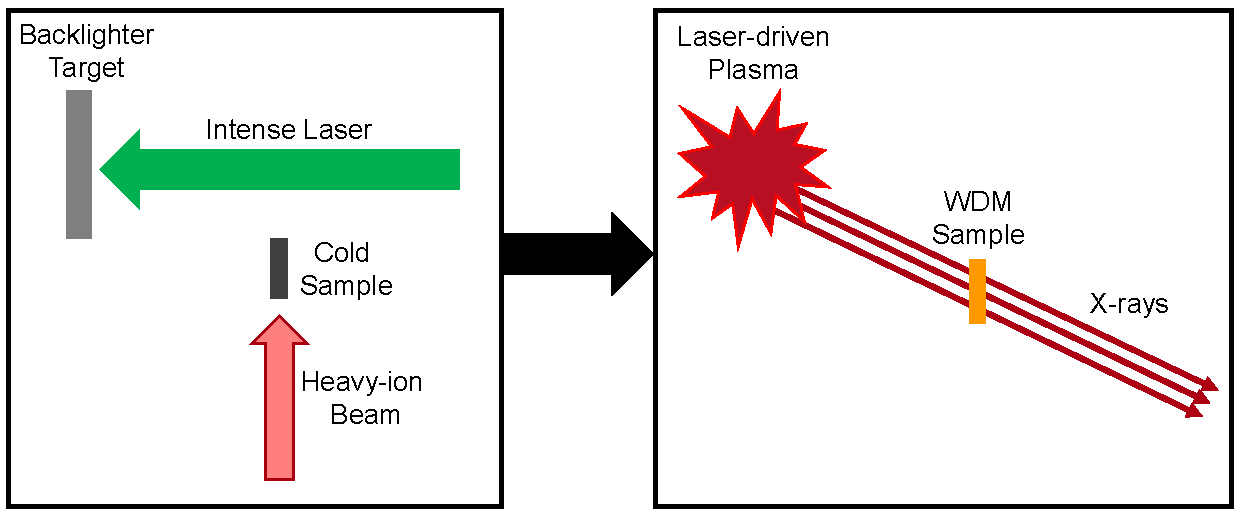
\includegraphics[width=0.85\textwidth]{Diagrams/HIHEX.pdf}
	\caption{Schematic of experiment using heavy ions for WDM generation paired with laser-driven X-ray sources for diagnostics.}
	\label{fig: HIHEX scheme}
\end{figure}

A project utilizing this scheme will be realized at the Facility for Antiproton and 
Ion Research (FAIR), an accelerator facility under 
construction in Darmstadt, Germany 
\cite{schoenberg2020high}, with current research work carried out at a 
neighboring facility, the GSI 
Helmholtz Center for Heavy Ion Research 
\citep{bagnoud2010commissioning}. With the goal of validating the experimental setup and demonstrating a proof of concept, preparatory experiments are conducted at the High energy, High 
Temperature (HHT) experimental station, where high-energy nanosecond laser pulses
from the Petawatt 
High-Energy Laser for Heavy Ion Experiments (PHELIX) 
are combined with heavy-ion beams originating at the 
UNIversal Linear ACcelerator (UNILAC) and accelerated 
by the heavy ion synchrotron SIS-18. Using these 
heavy-ion beams with velocities of 0.9 $c$
\cite{GSI_2023}, ion counts of $\sim 4\cdot 10^9$ 
for U$^{73+}$ per FWHM = \SI{100}{\nano\second} 
bunch, and an ion focal spot of 
$\sim$1$\times$\SI{1}{\milli\meter\squared}
\citep{GSI_2023_ion_num}, along with PHELIX ns-pulses 
with laser energies of up to 
\SI{200}{\joule} at 2$\omega$ (\SI{527}{\nano\meter}) and focused down to \SI{25}{\micro\meter} (FWHM), 
heavy-ion heating experiments using x-rays from 
laser-driven plasma can be conducted. As such, GSI 
offers, as of writing this, the
unique ability to combine intense heavy-ion beams 
with high-energy ns laser pulses 
\citep{hoffmann2006frontiers}. These capabilities 
will be expanded in the 
future at the Atomic, Plasma Physics and Applications 
(APPA) cave at FAIR, in its final stage achieving ion 
numbers of up to $\sim 5\cdot10^{11}$ ions 
(U$^{73+}$) per bunch through acceleration in the 
synchrotron SIS-100 \citep{schoenberg2020high}. The 
APPA cave will combine this more 
intense heavy-ion beam with a laser system of 
comparable characteristics to PHELIX, finally 
reaching the WDM regime with temperature states of up 
to >\SI{10}{\electronvolt}
\citep{schoenberg2020high}. 

On the path towards the generation of WDM, an 
experiment at HHT using the heavy-ions of the SIS-18 
synchrotron is planned for 2024, 
aiming to 
investigate heavy-ion heated Al samples through 
absorption 
spectroscopy around the Al K-edge. The work of this 
thesis is carried out in the context of a 
preparatory experiment conducted in May, 2023, 
whose goal is to investigate and optimize
the laser-driven x-ray backlighter and XAFS diagnostics setup in a 
laser-only beamtime using PHELIX.

Essential to the proposed experiments are x-ray spectrometers, which act as the primary measurement devices. By the nature of x-ray-matter interactions, conventional optical components, like lenses and mirrors, cannot be used for x-ray diagnostics. In the case of x-ray spectrometers, the number of refracting surfaces is usually limited to one, as otherwise rays are too heavily absorbed \citep{kunze2009introduction}. This restriction, as well as the violent conditions inherent to WDM experiments and the requirement of two well aligned spectra for deriving the Al absorption spectrum for XAFS, necessitate the design of spectrometers unique to this application. As such, my task is the design, implementation, and characterization of soft x-ray spectrometers to conduct XAFS of the Al K-edge by producing high resolution, high signal-to-noise ratio spectra, while accounting for the challenges inherent to the experimental setup.

Due to the prevalence of x-ray diagnostics in high-energy density matter research, x-ray spectrometers have become ubiquitous in the field and are now a well-matured technology \citep{renner2019challenges}. As is typical for the realm of high-resolution x-ray 
spectroscopy of extreme-state matter, crystals serve as the spectrally dispersing elements of the spectrometers. A deciding factor in the performance of these instruments is the shape of the crystal. In general, flat crystals offer simplicity of design and fewer defects in the crystal structure, while bent crystals enable focusing of the rays, leading to higher flexibility in the design, improved signal-to-noise ratios, and potential for better resolution, at the cost of increased complexity and introduction of crystal defects \citep{renner2019challenges,kunze2009introduction}. Drawing inspiration from 
spectrometers successfully implemented in other XAFS 
experiments \citep{levy2010double, 
torchio2016probing, hall1988experimental}, I created two soft x-ray spectrometers. The first targets the near-edge structures of XAFS and uses a 
dual channel, flat crystal geometry, while the second is intended 
for EXAFS and implements a focusing geometry, known 
as a Focusing Spectrograph with with Spatial 
Resolution (FSSR), with a 
spherically bent crystal. With these two starkly different constellations, I will weigh two contrasting design philosophies. On one hand, the flat crystal spectrometer focuses on ease of use and reliability, intending to reduce the overall complexity of the experimental setup and ensure best possible crystal quality. On the other, the bent crystal design emphasizes spectrometer performance, yielding potentially improved spectra and greater adaptability, but also adding complexity and chances for unforeseen difficulties. In the course of this thesis, each aspect of the spectrometers and their performance in the 2023 beamtime will be assessed and used to inform the design of spectrometers for future experiments.

This work is structured as follows. In chapter \ref{chapter: XAFS}, I discuss XAFS in depth and briefly present two experiments found in the literature which apply XAFS in WDM research. In chapter \ref{section: theory}, I explain the fundamentals of x-ray spectrometers, 
outlining the theory behind them with special focus 
placed on the FSSR. For the FSSR, I collect the 
sometimes inconsistent information from the 
literature and reformulate it to present a unified 
picture. I also derive the 
analytical dispersion of the spectrometer geometries relevant for 
this work and elaborate 
on resolution. In chapter \ref{chapter: spectrometer design}, the considerations and 
constraints placed on the spectrometer design 
according to their purpose and the experimental setup 
are listed and explained, followed by descriptions and explanations of the spectrometers' features in detail. In chapter \ref{chapter: experimental setup}, I present the experimental setup of the 2023 laser-only experiment at HHT, along with a description of the spectrometers' mechanical design and functions. In chapter \ref{chapter: data analysis}, the spectrum extraction and analysis procedure of the experimental data are explained. In chapter \ref{chapter: results and discussion}, I present the results and discuss their implications for the spectrometers. Finally, in chapter \ref{chapter: outlook} I summarize the content and findings of this work and apply them to recommend a spectrometer design for a combined experiment in 2024. 





